\section{Environment Construction and Validation}
\label{app:generation}

\subsection{Domain construction profiles}

Prompts are assembled from scene-, task-, and query-level templates. Dynamic
labels, values, and answers are derived from the same semantic state and task
execution recorded in the instance trace. The profiles below therefore
summarize the domain-specific state representations, rendering conventions,
and visible vocabularies; the common generation and reward pipeline is
described in Section~\ref{sec:design}.

\paragraph{Charts.}
Chart scenes are constructed from procedural marks, axes, scales, legends, and
panels spanning Cartesian, radial, geographic, flow, tabular, and compositional
layouts. Rendering controls vary chart treatment, palette, typography, tick
density, mark style, and compatible report context without modifying the
underlying data. Curated entity, temporal, scientific, and compact label pools
provide distinct series, category, panel, and region names within each figure.

\paragraph{Games.}
Game scenes combine procedural boards, tracks, hands, scores, pieces, enemies,
and action states with curated cards, dice, tokens, and sprite-like assets.
Each renderer follows the layout and interaction rules of its scene grammar
rather than a shared generic board template. Coordinates, score displays,
status labels, and action cues are derived from the simulated state, while
optional interface overlays and surface treatments provide visual variation.

\paragraph{Geometry.}
Geometry scenes are generated from analytic constructions of points, lines,
angles, polygons, circles, solids, coordinate systems, and measurement
instruments under solved numeric constraints. Textbook, whiteboard, and
technical-diagram profiles vary stroke, shading, notation placement, and
typography. Point labels, measurements, equations, and answer options are bound
after construction so that the visible diagram and symbolic problem statement
remain consistent with the same geometric state.

\paragraph{Graphs.}
Graph scenes begin with explicit nodes, edges, weights, paths, and state
transitions, which are then realized through circular, layered, tree, route, or
force-directed layouts. Node shape, edge style, palette, and framing vary
independently of topology. Numeric, alphabetic, and named node vocabularies are
sampled without collisions, and labels and edge values remain attached to
their semantic elements across layout changes.

\paragraph{Icons.}
Icon scenes populate fields, grids, paths, rings, paired canvases, and rendered
option sets with curated icon assets. Procedural controls vary icon identity,
color, scale, rotation, spacing, ordering, and transformation while preserving
legibility and answer uniqueness. Marker and option labels are placed as part
of the scene geometry, allowing counting, adjacency, transformation, and
matching tasks to share a consistent visual vocabulary.

\paragraph{Illustrations.}
Illustration scenes compose semantic object, part, and tile catalogs into
rooms, construction sites, libraries, tactical maps, and isometric
environments. Scene-specific layout rules determine occupancy, overlap, depth,
and permitted object relations, after which palette, asset, framing, and
surface treatments vary the appearance. Explicit tile, object, and option
labels are introduced only when required by the task program.

\paragraph{Pages.}
Page scenes represent structured records through forms, tables, calendars,
schedules, application controls, documents, and infographic components.
Templates govern visual hierarchy, alignment, interface framing, spacing, and
typography, while information-density and context profiles vary the
presentation. Field names, section headings, dates, values, and control labels
remain linked to the underlying document state.

\paragraph{Physics.}
Physics scenes assemble apparatus, forces, wires, rays, fields, graphs, and
measurement instruments from explicit physical quantities and component
states. Technical-diagram profiles vary line work, component treatment,
background, and label placement while preserving the solved configuration.
Quantities, units, directions, and component names are rendered from the same
state used by formula-evaluation, comparison, and state-update programs.

\paragraph{Puzzles.}
Puzzle scenes include rule-governed grids, mazes, pipes, matrices, nets, voxel
boards, and candidate sets sampled under validity and uniqueness constraints.
Symbols, board skins, spacing, missing-cell treatments, and option scaffolds
vary the presentation without revealing the underlying rule. Coordinates,
candidate labels, and compact clues are added only when required by the puzzle
definition or answer interface.

\paragraph{Symbolic.}
Symbolic scenes use notation-specific generators for clocks, abaci, dice,
spinners, musical staves, logic circuits, formal tables, tapes, and encoded
glyph systems. Symbols and transitions are represented as executable state
rather than decorative text. Fonts, notation cards, palettes, spacing, and
layout may vary, while tokens, values, note names, and state labels remain
bound to the formal structure being queried.

\paragraph{Three-dimensional scenes.}
Three-dimensional scenes arrange procedural meshes and object assets under
explicit camera, projection, depth, occlusion, and surface constraints.
Viewpoint, material, lighting, ground or wall treatment, and framing vary
without changing the queried spatial relation. Object, lane, wall, point, and
candidate labels are placed after projection and checked against the final
image geometry for visibility and separation.

\subsection{Operation-family definitions}
\label{app:operation-families}

Figure~\ref{fig:operation-coverage} classifies tasks according to the
operations that materially contribute to their outputs. Assignments are
multi-label when a task program composes several operations.

\textit{Direct retrieval} denotes a localized visible lookup for which no
other substantive operation determines the answer. \textit{Filtering}
constructs a subset using a predicate, relation, or named scope, and
\textit{counting} returns the cardinality of such a set. \textit{Comparison}
evaluates equality, order, thresholds, or intervals, whereas \textit{ranking}
orders candidates or selects an extremum or ordinal item.
\textit{Aggregation} reduces a collection using a sum, mean, median,
cumulative total, share, mass, or related statistic.

\textit{Logical composition} combines predicates or sets through conjunction,
disjunction, negation, union, intersection, or difference.
\textit{Spatial relations} covers positional, directional, metric, overlap,
containment, and occlusion relations. \textit{Topology} covers connectivity,
paths, components, cycles, traversal, and reachability.
\textit{Matching} evaluates equivalence, correspondence, consistency,
completion, or candidate-to-reference agreement.

\textit{Transformation} applies or infers a geometric, symbolic,
representational, folding, projection, overlay, or reconstruction operation.
\textit{State update} applies a move, action, counterfactual edit, or discrete
transition. \textit{Formula evaluation} uses arithmetic, algebra, a
domain-specific formula, a derived metric, or a numeric difference, ratio, or
rate.

\subsection{Invariant enforcement}

Semantic generation first enforces task-specific constraints and answer
uniqueness. Structural realization is completed before geometry-dependent
verifier state is projected into image coordinates, and post-render effects
preserve the final canvas coordinate system. Render-only controls may not
modify task-program operands, answer values, or the reward contract.

Independent seeded streams and the recorded instance trace allow the semantic
state, prompt, rendering choices, and verifier state to be replayed together.
The precise ordering of optional finishing layers remains renderer-specific.
Table~\ref{tab:variation-layers} summarizes the variation levels and their
required invariants.

\begin{table}[t]
  \centering
  \scriptsize
  \setlength{\tabcolsep}{3.5pt}
  \renewcommand{\arraystretch}{1.02}
  \caption{Variation layers and the invariants they preserve.}
  \label{tab:variation-layers}
  \begin{tabular}{@{}>{\raggedright\arraybackslash}p{0.21\linewidth}
                       >{\raggedright\arraybackslash}p{0.44\linewidth}
                       >{\raggedright\arraybackslash}p{0.25\linewidth}@{}}
    \toprule
    Layer & Representative controls & Required invariant \\
    \midrule
    Semantic instance
      & Dimensions, cardinalities, values, operation length, candidate set
      & Scene grammar and task program \\
    Structural realization
      & Placement, spacing, panel arrangement, framing, answer-preserving camera
      & Semantic relations and answer \\
    Surface and context
      & Palette, typography, skins, materials, labels, non-answer text
      & Semantic state and answer \\
    Post-render
      & Blur, resampling, compression, tone, noise, texture
      & Canvas geometry and answer \\
    \bottomrule
  \end{tabular}
\end{table}


Figure~\ref{fig:rendering-pipeline} illustrates how semantic execution,
structural realization, projection, and surface treatment interact while
preserving the task output.

\begin{figure}[t]
  \centering
  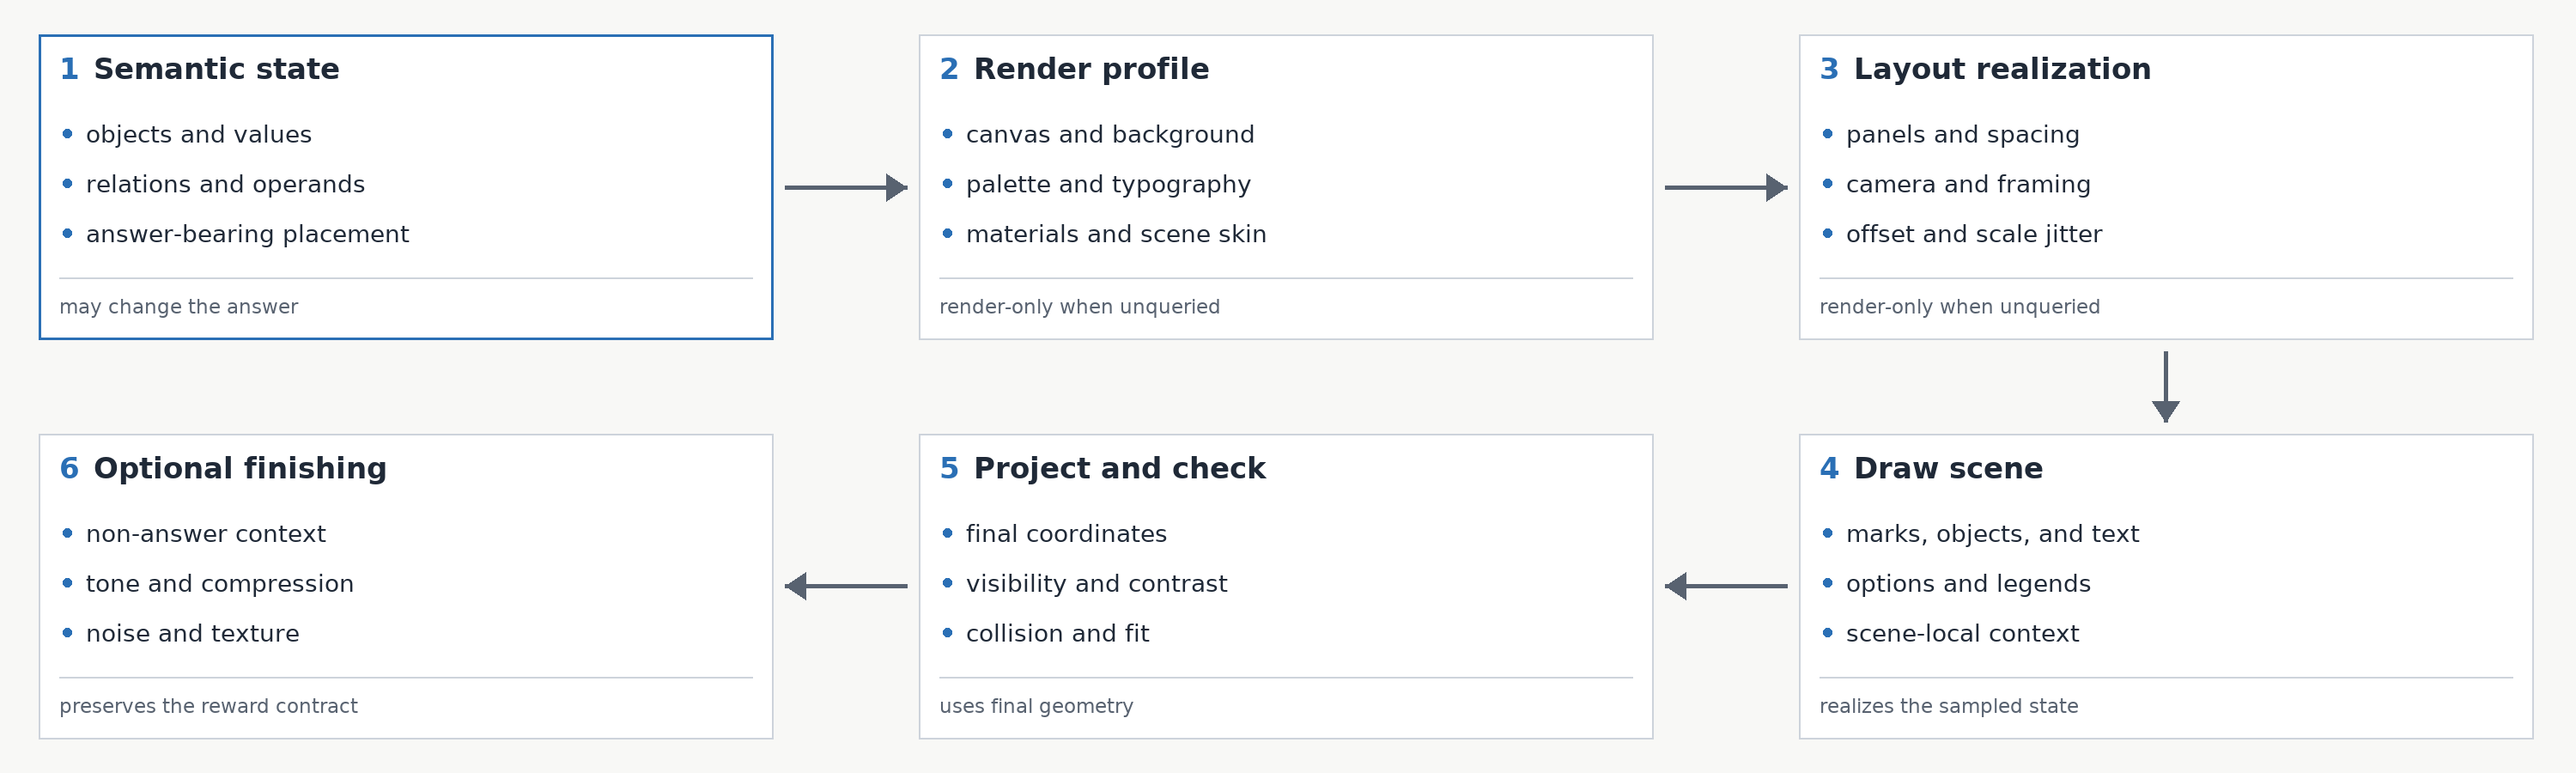
\includegraphics[width=0.9\textwidth]{figures/rendering_variation_pipeline.png}
  \caption{Control flow for visual realization. Structural and surface
  controls are treated as render-only when they preserve the queried semantic
  relations and typed answer. Answer-bearing geometry is projected before
  validation, while optional context and raster finishing remain
  scene-specific and are recorded in the instance trace.}
  \label{fig:rendering-pipeline}
\end{figure}

Table~\ref{tab:rendering-variation-profiles} specifies the controlled
realizations used in Figure~\ref{fig:rendering-variation}.

% Generated by paper/trace/scripts/build_method_figures.py; do not edit manually.
\begin{table}[h]
  \centering
  \scriptsize
  \setlength{\tabcolsep}{4pt}
  \renewcommand{\arraystretch}{1.08}
  \caption{Controlled profiles in the fixed-instance rendering sweep.}
  \label{tab:rendering-variation-profiles}
  \begin{tabular}{@{}p{0.18\linewidth}p{0.18\linewidth}p{0.53\linewidth}@{}}
    \toprule
    Profile & Controlled axis & Realization \\
    \midrule
    Baseline & Reference & Light neutral theme, sans-serif type, fixed layout, no context or noise \\
    Color palette & Palette & Warm editorial palette; graph topology and layout retained \\
    Typeface & Typography & EB Garamond node-label typeface; baseline palette and layout retained \\
    Layout & Structure & Circular node placement replaces the baseline spring layout \\
    Report context & Non-answer context & Curated paragraph context in reserved non-answer panel space \\
    Raster noise & Post-render & Gaussian noise with fixed sigma; coordinate geometry retained \\
    \bottomrule
  \end{tabular}
\end{table}



\section{Experimental Details}
\label{app:experiments}

Table~\ref{tab:training-configuration} reports the configuration shared by the
3B and 7B training runs.

% Generated by paper/trace/scripts/build_results_assets.py. Do not edit.
\begin{table}[t]
  \centering
  \small
  \setlength{\tabcolsep}{5pt}
  \caption{RLVR configuration shared across the 3B and 7B runs.}
  \label{tab:training-configuration}
  \begin{tabular}{@{}l l@{}}
    \toprule
    Setting & Value \\
    \midrule
    Training data & 64,000 prompts; 1,000 tasks \\
    Image pixel cap & 1,280,000 per image \\
    Updates & 500; one shuffled data pass \\
    Validation & 2,000 instances every 100 updates \\
    Prompt batch / rollouts & 128 / 8 \\
    Sampled responses & 512,000 \\
    Prompt / response caps & 2,048 / 2,048 tokens \\
    Optimization scope & Full model; vision encoder trainable; BF16 \\
    Actor optimizer & AdamW; LR $10^{-6}$; weight decay 0.01 \\
    Policy epochs & 1 \\
    Policy clipping & 0.2 lower; 0.3 upper; dual 3.0 \\
    Rollout sampling & temperature 1.0; top-$p$ 1.0 \\
    Reward & 0.95 exact answer $+$ 0.05 JSON format \\
    Hardware & 8 $\times$ H100 80GB \\
    Runtime & 12.2 h (3B); 13.9 h (7B) \\
    \bottomrule
  \end{tabular}
\end{table}


External inference uses temperature 0.6, top-$p$ 1.0, a 4,096-token response
limit, and decoding seeds 42, 43, and 44. The seeds affect response generation
only; model weights remain fixed across decoding runs.

\subsection{\trace validation slices}

Table~\ref{tab:iid-slice-results} reports held-out \trace accuracy by answer
interface and query structure. Each task contributes two previously unseen
instances, and all slice scores use one decoding seed. The rows are overlapping
analytical views of the same task inventory rather than separate evaluation
sets.

% Generated by paper/trace/scripts/build_iid_taxonomy_analysis.py. Do not edit.
\begin{table}[t]
  \centering
  \fontsize{7.5}{8.6}\selectfont
  \setlength{\tabcolsep}{4.8pt}
  \caption{Accuracy by answer interface and query structure on the 2,000-instance \trace validation set. Each task contributes two unseen instances and scores use one decoding seed. Rows are analytical slices of the same task inventory.}
  \label{tab:iid-slice-results}
  \begin{tabular}{@{}l c c c c c c c@{}}
    \toprule
    & & \multicolumn{3}{c}{3B} & \multicolumn{3}{c}{7B} \\
    \cmidrule(lr){3-5}\cmidrule(l){6-8}
    Slice & Tasks & Base & After RLVR & $\Delta$ & Base & After RLVR & $\Delta$ \\
    \midrule
    \multicolumn{8}{@{}l}{\textit{Answer interface}} \\
    Integer & 547 & 22.39 & 37.84 & +15.45 & 30.35 & 49.36 & +19.01 \\
    Numeric & 51 & 24.51 & 95.10 & +70.59 & 49.02 & 94.12 & +45.10 \\
    Option letter & 210 & 26.43 & 30.95 & +4.52 & 33.33 & 40.48 & +7.14 \\
    String & 192 & 28.12 & 46.88 & +18.75 & 42.45 & 58.59 & +16.15 \\
    \midrule
    \multicolumn{8}{@{}l}{\textit{Query structure}} \\
    Single-query tasks & 683 & 24.52 & 39.82 & +15.30 & 33.53 & 50.88 & +17.35 \\
    Multi-query tasks & 317 & 24.29 & 43.69 & +19.40 & 35.80 & 53.00 & +17.19 \\
    \bottomrule
  \end{tabular}
\end{table}


\subsection{External evaluation suite}

Each benchmark is evaluated with its standard scorer when available. A small
number of open-answer benchmarks retain their fixed model-based grading
procedures; the same grader, prompt, and parser are used for every checkpoint.
Table~\ref{tab:evaluation-suite} lists the complete benchmark suite, references,
and evaluated sample counts.

% Generated by paper/trace/scripts/build_results_assets.py. Do not edit.
\begin{table}[t]
  \centering
  \scriptsize
  \setlength{\tabcolsep}{4pt}
  \caption{External evaluation suite. Each model and decoding seed is scored on 32,805 examples.}
  \label{tab:evaluation-suite}
  \begin{tabular}{@{}p{0.30\textwidth} p{0.38\textwidth} c@{}}
    \toprule
    Category & Benchmark & Rows \\
    \midrule
    Charts \& Tables & ChartQAPro~\citep{masry2025chartqapro} & 1,948 \\
     & CharXivReason~\citep{wang2024charxiv} & 1,000 \\
     & TableVQABench~\citep{kim2024tablevqabench} & 1,500 \\
     & EvoChart~\citep{huang2025evochart} & 1,250 \\
    \midrule
    Visual Math & MathVision~\citep{wang2024mathvision} & 3,040 \\
     & MathVista~\citep{lu2024mathvista} & 1,000 \\
     & MathVerse~\citep{zhang2024mathverse} & 788 \\
     & WeMath~\citep{qiao2025wemath} & 1,740 \\
    \midrule
    Science \& General & PhyX mini MC~\citep{shen2025phyx} & 1,000 \\
     & MMMU-ProVis~\citep{yue2025mmmupro} & 1,730 \\
     & RealWorldQA~\citep{xai2024realworldqa} & 765 \\
     & MMStar~\citep{chen2024mmstar} & 1,500 \\
    \midrule
    Spatial Reasoning & EmbSpatial~\citep{du2024embspatial} & 3,640 \\
     & SpatialVizBench~\citep{wang2026spatialviz} & 1,180 \\
     & CV-Bench 3D~\citep{tong2024cambrian} & 1,200 \\
     & ERQA~\citep{deepmind2025erqa} & 400 \\
    \midrule
    Perception \& Counting & BLINK~\citep{fu2024blink} & 1,901 \\
     & CountBenchQA~\citep{paiss2023countbench} & 487 \\
     & CountQA~\citep{tamarapalli2025countqa} & 1,528 \\
     & TreeBench~\citep{wang2026treebench} & 405 \\
    \midrule
    Puzzles \& Logic & PuzzleVQA~\citep{chia2024puzzlevqa} & 2,000 \\
     & VisualPuzzles~\citep{song2025visualpuzzles} & 1,168 \\
     & LogicVista~\citep{xiao2024logicvista} & 447 \\
     & MME-Reasoning~\citep{yuan2025mmereasoning} & 1,188 \\
    \bottomrule
  \end{tabular}
\end{table}


\subsection{External benchmark uncertainty}

Table~\ref{tab:external-bootstrap-cis} reports paired confidence intervals for
the improvement from each base checkpoint to its \trace-trained counterpart.
For each bootstrap replicate, evaluation items are resampled jointly with the
predictions from all three decoding seeds. Benchmarks with grouped metrics are
resampled at their official scoring unit: problem families for WeMath and
items within official splits for TableVQABench.

% Generated by paper/trace/scripts/build_external_bootstrap_cis.py. Do not edit.
\begin{table}[t]
  \centering
  \fontsize{8.5}{9.5}\selectfont
  \setlength{\tabcolsep}{5pt}
  \renewcommand{\arraystretch}{1.10}
  \caption{Paired Base-to-\trace improvements on the external evaluation suite, in percentage points. Intervals are 95\% bootstrap percentile intervals, computed from the 2.5th and 97.5th percentiles of 10,000 paired item-bootstrap replicates; each sampled item carries results from all three decoding seeds. Bold intervals exclude zero. These intervals quantify variation over evaluation items rather than independently trained checkpoints.}
  \label{tab:external-bootstrap-cis}
  \begin{tabularx}{\textwidth}{@{}>{\raggedright\arraybackslash}p{0.20\textwidth} *{4}{>{\centering\arraybackslash}X}@{}}
    \toprule
    & \multicolumn{2}{c}{3B} & \multicolumn{2}{c}{7B} \\
    \cmidrule(lr){2-3}\cmidrule(l){4-5}
    Benchmark & $\Delta$ & 95\% CI & $\Delta$ & 95\% CI \\
    \midrule
    \rowcolor{TraceChartsBand} \multicolumn{5}{@{}l@{}}{\textbf{Charts \& Tables}} \\
    \rowcolor{TraceChartsBand} ChartQAPro & $-0.14$ & $[-1.30,\ +1.06]$ & $+2.24$ & \textbf{$[+0.76,\ +3.66]$} \\
    \rowcolor{TraceChartsBand} CharXivReason & $+5.77$ & \textbf{$[+4.13,\ +7.40]$} & $+7.40$ & \textbf{$[+5.33,\ +9.50]$} \\
    \rowcolor{TraceChartsBand} TableVQABench & $+2.72$ & \textbf{$[+1.78,\ +3.69]$} & $+3.11$ & \textbf{$[+2.01,\ +4.21]$} \\
    \rowcolor{TraceChartsBand} EvoChart & $-1.68$ & \textbf{$[-3.20,\ -0.16]$} & $+7.84$ & \textbf{$[+5.89,\ +9.79]$} \\
    \specialrule{0.35pt}{0pt}{0pt}
    \rowcolor{TraceMathBand} \multicolumn{5}{@{}l@{}}{\textbf{Visual Math}} \\
    \rowcolor{TraceMathBand} MathVision & $+6.10$ & \textbf{$[+5.02,\ +7.18]$} & $+2.61$ & \textbf{$[+1.54,\ +3.66]$} \\
    \rowcolor{TraceMathBand} MathVista & $+6.30$ & \textbf{$[+4.53,\ +8.07]$} & $+4.70$ & \textbf{$[+2.80,\ +6.53]$} \\
    \rowcolor{TraceMathBand} MathVerse & $+6.43$ & \textbf{$[+4.27,\ +8.54]$} & $+4.31$ & \textbf{$[+2.12,\ +6.56]$} \\
    \rowcolor{TraceMathBand} WeMath & $+10.95$ & \textbf{$[+8.73,\ +13.24]$} & $+10.96$ & \textbf{$[+8.39,\ +13.56]$} \\
    \specialrule{0.35pt}{0pt}{0pt}
    \rowcolor{TraceScienceBand} \multicolumn{5}{@{}l@{}}{\textbf{Science \& General}} \\
    \rowcolor{TraceScienceBand} PhyX mini MC & $+4.67$ & \textbf{$[+3.40,\ +5.90]$} & $+7.73$ & \textbf{$[+5.10,\ +10.37]$} \\
    \rowcolor{TraceScienceBand} MMMU-ProVis & $+4.57$ & \textbf{$[+3.12,\ +6.05]$} & $+3.66$ & \textbf{$[+2.22,\ +5.13]$} \\
    \rowcolor{TraceScienceBand} RealWorldQA & $+1.79$ & \textbf{$[+0.92,\ +2.66]$} & $+3.05$ & \textbf{$[+1.44,\ +4.71]$} \\
    \rowcolor{TraceScienceBand} MMStar & $+2.98$ & \textbf{$[+1.93,\ +4.04]$} & $+3.76$ & \textbf{$[+2.44,\ +5.16]$} \\
    \specialrule{0.35pt}{0pt}{0pt}
    \rowcolor{TraceSpatialBand} \multicolumn{5}{@{}l@{}}{\textbf{Spatial Reasoning}} \\
    \rowcolor{TraceSpatialBand} EmbSpatial & $+1.81$ & \textbf{$[+1.34,\ +2.28]$} & $+1.53$ & \textbf{$[+0.94,\ +2.09]$} \\
    \rowcolor{TraceSpatialBand} SpatialVizBench & $+1.75$ & $[-0.28,\ +3.84]$ & $+0.54$ & $[-1.64,\ +2.85]$ \\
    \rowcolor{TraceSpatialBand} CV-Bench 3D & $+8.31$ & \textbf{$[+6.50,\ +10.11]$} & $+4.75$ & \textbf{$[+3.11,\ +6.39]$} \\
    \rowcolor{TraceSpatialBand} ERQA & $+1.08$ & $[-0.50,\ +2.75]$ & $+2.17$ & $[-0.17,\ +4.50]$ \\
    \specialrule{0.35pt}{0pt}{0pt}
    \rowcolor{TracePerceptionBand} \multicolumn{5}{@{}l@{}}{\textbf{Perception \& Counting}} \\
    \rowcolor{TracePerceptionBand} BLINK & $+2.61$ & \textbf{$[+1.75,\ +3.49]$} & $+3.26$ & \textbf{$[+2.03,\ +4.54]$} \\
    \rowcolor{TracePerceptionBand} CountBenchQA & $+3.22$ & \textbf{$[+1.85,\ +4.65]$} & $+2.67$ & \textbf{$[+1.03,\ +4.31]$} \\
    \rowcolor{TracePerceptionBand} CountQA & $+0.76$ & $[-0.07,\ +1.59]$ & $+2.92$ & \textbf{$[+1.44,\ +4.43]$} \\
    \rowcolor{TracePerceptionBand} TreeBench & $-0.66$ & $[-2.47,\ +1.15]$ & $+2.22$ & $[+0.00,\ +4.44]$ \\
    \specialrule{0.35pt}{0pt}{0pt}
    \rowcolor{TracePuzzlesBand} \multicolumn{5}{@{}l@{}}{\textbf{Puzzles \& Logic}} \\
    \rowcolor{TracePuzzlesBand} PuzzleVQA & $+6.58$ & \textbf{$[+4.90,\ +8.23]$} & $+5.45$ & \textbf{$[+3.85,\ +7.08]$} \\
    \rowcolor{TracePuzzlesBand} VisualPuzzles & $+2.31$ & \textbf{$[+0.37,\ +4.22]$} & $+2.94$ & \textbf{$[+0.88,\ +4.97]$} \\
    \rowcolor{TracePuzzlesBand} LogicVista & $+3.65$ & \textbf{$[+0.45,\ +6.79]$} & $+4.70$ & \textbf{$[+1.42,\ +7.98]$} \\
    \rowcolor{TracePuzzlesBand} MME-Reasoning & $+2.44$ & \textbf{$[+0.76,\ +4.07]$} & $+2.86$ & \textbf{$[+1.04,\ +4.69]$} \\
    \bottomrule
  \end{tabularx}
\end{table}


% Generated by scripts/build_scene_atlas.py; do not edit by hand.
\section{Representative Task Atlas}
\label{app:task-atlas}

Each page presents twelve seeded examples from one visual domain. Panels pair each rendered instance with its semantic question and typed answer. Rule-heavy questions are condensed only when required for legibility.

\begingroup
\setlength{\fboxsep}{2pt}
\setlength{\fboxrule}{0.3pt}
\definecolor{traceatlasborder}{HTML}{D1D5DB}
\definecolor{traceatlasanswer}{HTML}{2A6FB5}
\newcommand{\traceatlaspromptnormal}{\fontsize{5.5}{6.0}\selectfont}
\newcommand{\traceatlaspromptdense}{\fontsize{4.75}{5.2}\selectfont}
\newcommand{\traceatlascard}[5]{%
  \begingroup
  \color{traceatlasborder}%
  \fbox{%
    \color{black}%
    \begin{minipage}[t][0.176\textheight][t]{0.298\textwidth}
      \raggedright\setlength{\parindent}{0pt}%
      {\fontsize{5.1}{5.6}\selectfont\sffamily\color{gray}\textbf{#1}\par}%
      \vspace{1pt}%
      \centering\includegraphics[width=\linewidth,height=0.088\textheight,keepaspectratio]{#2}\par
      \vspace{1pt}%
      \raggedright{\sffamily #5 #3\par}%
      \vfill
      {\fontsize{5.6}{6.1}\selectfont\sffamily\color{traceatlasanswer}\textbf{Answer: #4}\par}%
    \end{minipage}%
  }%
  \endgroup
}

\begin{figure}[p]
\centering
\traceatlascard{Error Interval: Reference Containment}{figures/scene_atlas/assets/charts_01_error_interval_reference_containment_count.png}{The image shows a horizontal interval chart with labeled categories, point estimates, and lower-to-upper interval whiskers. Count the intervals whose lower-to-upper span contains reference value 54.}{4}{\traceatlaspromptnormal}
\hfill
\traceatlascard{Region Map: Numeric Interval Region}{figures/scene_atlas/assets/charts_02_region_map_numeric_interval_region_count.png}{This image shows a world map with selected countries colored by value and a color legend. What number of countries fall in value bins between 20 and 99, inclusive?}{6}{\traceatlaspromptnormal}
\hfill
\traceatlascard{Scatter Cluster: Centroid Option Selection}{figures/scene_atlas/assets/charts_03_scatter_cluster_centroid_option_selection_label.png}{The visual shows a scatter plot with several colored point clusters and a matching legend. Find the centroid of cluster "Milow" by eye. Which option marker is closest?}{A}{\traceatlaspromptnormal}
\par\vspace{2pt}
\noindent
\traceatlascard{Size Encoding: Panel Category Extremum Panel}{figures/scene_atlas/assets/charts_04_size_encoding_panel_category_extremum_panel_label.png}{The image shows multiple packed bubble-chart panels where bubble size indicates value and color indicates category. For category "River", which panel contains the item with the largest size?}{Delta}{\traceatlaspromptnormal}
\hfill
\traceatlascard{Scatter Points: Category Threshold Point}{figures/scene_atlas/assets/charts_05_scatter_points_category_threshold_point_count.png}{The chart shows a categorized scatter plot with individual data points, numeric x- and y-axes, and a legend. How many plotted points from category "Storage" satisfy x greater than 50?}{2}{\traceatlaspromptnormal}
\hfill
\traceatlascard{Single Series: Threshold Value}{figures/scene_atlas/assets/charts_06_single_series_threshold_value_count.png}{The image shows an ordered labeled dot plot where point labels identify y-values from left to right. Determine how many marks show values strictly greater than 19.}{10}{\traceatlaspromptnormal}
\par\vspace{2pt}
\noindent
\traceatlascard{Population Pyramid: Age Group Threshold}{figures/scene_atlas/assets/charts_07_population_pyramid_age_group_threshold_count.png}{The image shows a mirrored horizontal bar chart with one row per age group. The left and right bars show the two legend series on the same positive scale. Using the two bar values in each row, how many age groups satisfy: the sum of "Urban" and "Rural" at most 140?}{3}{\traceatlaspromptdense}
\hfill
\traceatlascard{Area: Stacked Band Dominance}{figures/scene_atlas/assets/charts_08_area_stacked_band_dominance_label.png}{The visual shows one stacked area chart with colored category bands, numeric band values, and a legend. Sum each category's band values over "S9W6" through "H2W5" in displayed x-axis order; which category is largest?}{Tradd}{\traceatlaspromptnormal}
\hfill
\traceatlascard{Annotated Series: Callout Endpoint Change}{figures/scene_atlas/assets/charts_09_annotated_series_callout_endpoint_change_value.png}{The figure shows a labeled line chart with one visible annotation. Compare the callout mark with "Hari". What is the nonnegative difference between their values?}{7}{\traceatlaspromptnormal}
\par\vspace{2pt}
\noindent
\traceatlascard{Combo Mark: Conditioned Line Extremum}{figures/scene_atlas/assets/charts_10_combo_mark_conditioned_line_extremum_label.png}{The figure shows stacked bars for "Nimbus" with an overlaid line for "Birch"; each category displays the relevant printed values. First keep categories with "Nimbus" greater than 55; which remaining category has the maximum "Birch" value?}{QV2}{\traceatlaspromptdense}
\hfill
\traceatlascard{Uncertainty Band: Band Overlap}{figures/scene_atlas/assets/charts_11_uncertainty_band_band_overlap_count.png}{The image shows a line chart with two labeled series, each shown with a central line and a shaded upper-to-lower uncertainty band. At how many x-axis labels do the shaded bands for "Direct" and "Antimony" overlap?}{1}{\traceatlaspromptnormal}
\hfill
\traceatlascard{Matrix: Off Diagonal Confusion}{figures/scene_atlas/assets/charts_12_matrix_off_diagonal_confusion_label.png}{The figure shows a labeled confusion matrix with printed integer counts in each active cell. In the row for actual class "Tartus", exclude the matching diagonal cell. What predicted column label has the largest count?}{Namanga}{\traceatlaspromptnormal}
\caption{Representative chart tasks.}
\label{fig:task-atlas-charts}
\end{figure}
\clearpage

\begin{figure}[p]
\centering
\traceatlascard{Sokoban: Box Goal Status}{figures/scene_atlas/assets/games_01_sokoban_box_goal_status_count.png}{The figure shows a Sokoban board with walls, a player, colored boxes, and colored goal dots; a box on its matching goal has the goal dot drawn on top of the box. How many boxes are not on their matching colored goal dots?}{3}{\traceatlaspromptdense}
\hfill
\traceatlascard{Checkers: Max Capture Chain Length}{figures/scene_atlas/assets/games_02_checkers_max_capture_chain_length.png}{Red moves on the shown 8 by 8 checkers board. A jump captures an adjacent opponent and lands on the empty square beyond. The marked piece is a king, so it may jump diagonally in either direction and continue while another capture is available. What is its maximum capture-chain length?}{2}{\traceatlaspromptdense}
\hfill
\traceatlascard{Darts: Dart Score}{figures/scene_atlas/assets/games_03_darts_dart_score_value.png}{The image shows a simplified labeled dartboard with visible dart markers. Using the simplified dartboard scoring rule, what is the dart's score? A dart in a numbered sector scores that number; a dart in the center bullseye scores 50.}{7}{\traceatlaspromptdense}
\par\vspace{2pt}
\noindent
\traceatlascard{Pacman: Next Item}{figures/scene_atlas/assets/games_04_pacman_next_item_label.png}{This scene shows a Pac-Man style maze with a visible Pac-Man marker, ghosts, normal pellets, bonus items, and a highlighted route. Among the labeled bonus items, which one is encountered first on the highlighted route?}{F}{\traceatlaspromptnormal}
\hfill
\traceatlascard{Minesweeper: Forced Cell}{figures/scene_atlas/assets/games_05_minesweeper_forced_cell_count.png}{In the Minesweeper grid, each number gives the mine count among its eight neighbors and each flag is a known mine. If a clue already has enough flags, its other hidden neighbors are safe; if every remaining hidden neighbor is needed, they are mines. From the outlined clue cells, how many hidden cells must be safe?}{5}{\traceatlaspromptdense}
\hfill
\traceatlascard{Chess: Target Square Attacker}{figures/scene_atlas/assets/games_06_chess_target_square_attacker_count.png}{The scene shows a partial chess board with white and black pieces. How many black pieces currently attack the red outlined target square?}{0}{\traceatlaspromptnormal}
\par\vspace{2pt}
\noindent
\traceatlascard{Reversi: Marked Move Flip}{figures/scene_atlas/assets/games_07_reversi_marked_move_flip_count.png}{White moves on the shown 8 by 8 Reversi board. A legal move brackets opponent discs along one or more straight lines, and all bracketed discs flip. How many discs flip after playing at the red marked square?}{4}{\traceatlaspromptdense}
\hfill
\traceatlascard{Bubble Shooter: Pop Color}{figures/scene_atlas/assets/games_08_bubble_shooter_pop_color_label.png}{A shot bubble attaches at the marked target. A connected same-color group pops when the placement makes its size at least three. Which option labels the bubble color that would pop a group there?}{D}{\traceatlaspromptdense}
\hfill
\traceatlascard{Snakes Ladders: Remaining To Finish}{figures/scene_atlas/assets/games_09_snakes_ladders_remaining_to_finish_value.png}{The visual shows a numbered Snakes and Ladders board with one token and visible snakes and ladders. How far is the token from the final square by square number?}{12}{\traceatlaspromptnormal}
\par\vspace{2pt}
\noindent
\traceatlascard{Racing Track: Ahead Object}{figures/scene_atlas/assets/games_10_racing_track_ahead_object_count.png}{The scene shows a top-down loop racing track with a checkered finish line, a direction arrow, a marked car, and other labeled cars. Follow the arrow direction from the marked car to the finish line. Do not count the marked car. Count only the cars ahead of the marked car before the finish line.}{0}{\traceatlaspromptdense}
\hfill
\traceatlascard{Circular Chess: Target Cell Reacher}{figures/scene_atlas/assets/games_11_circular_chess_target_cell_reacher_count.png}{On this four-ring, sixteen-sector circular chess board, sectors wrap but rings do not. The red cell is the target. Rooks move along or across rings, bishops diagonally, queens as both, knights jump, and kings one step; sliding pieces stop at the first occupied cell. How many Black pieces can reach the target?}{3}{\traceatlaspromptdense}
\hfill
\traceatlascard{Dots And Boxes: Owned Box}{figures/scene_atlas/assets/games_12_dots_and_boxes_owned_box_count.png}{The scene shows a dots-and-boxes grid with some edges already drawn. How many boxes are marked with player B?}{8}{\traceatlaspromptnormal}
\caption{Representative game tasks.}
\label{fig:task-atlas-games}
\end{figure}
\clearpage

\begin{figure}[p]
\centering
\traceatlascard{Circle Pair Tangents: External Tangent Segment Length}{figures/scene_atlas/assets/geometry_01_circle_pair_tangents_external_tangent_segment_length_value.png}{This geometry diagram shows two separated non-concentric circles with centers C and D, a common tangent touching them at A and B, radii to the tangent points, and an auxiliary right triangle CED whose leg ED shows the radius difference. Find the center-to-center distance CD.}{225}{\traceatlaspromptdense}
\hfill
\traceatlascard{Solid Cross Section: Square Pyramid Parallel Slice Area}{figures/scene_atlas/assets/geometry_02_solid_cross_section_square_pyramid_parallel_slice_area.png}{The labeled diagram shows a square pyramid cut by a plane parallel to its base, with the cross-section marked and dimensions labeled. The marked slice is parallel to the base. Use similar solids with scale d/H to find the value of A for the cross-section.}{130}{\traceatlaspromptdense}
\hfill
\traceatlascard{Measuring Tools: Protractor Angle}{figures/scene_atlas/assets/geometry_03_measuring_tools_protractor_angle_value.png}{The figure shows a geometric figure with a protractor placed at the marked angle. Read the protractor scale at the marked angle. What is the angle measure in degrees?}{150}{\traceatlaspromptnormal}
\par\vspace{2pt}
\noindent
\traceatlascard{Sector: Central Angle From Sector Measure}{figures/scene_atlas/assets/geometry_04_sector_central_angle_from_sector_measure_value.png}{The sector figure shows a circular sector with labeled points. Compute the measure of angle AOB. Use the labeled radius and shaded sector area.}{45}{\traceatlaspromptnormal}
\hfill
\traceatlascard{Special Quadrilateral: Segment Length}{figures/scene_atlas/assets/geometry_05_special_quadrilateral_segment_length_value.png}{The figure shows a quadrilateral with construction marks and measurement labels. Solve the visible rhombus side expressions. What is the length of "segment CD"?}{43}{\traceatlaspromptnormal}
\hfill
\traceatlascard{Paper Fold: Folded Segment Length}{figures/scene_atlas/assets/geometry_06_paper_fold_folded_segment_length_value.png}{This folded-paper diagram shows a folded paper corner with dashed original edges, a crease, a folded flap, and side-length labels. The crease EF folds A onto P. What is the value of the marked segment FP?}{231}{\traceatlaspromptnormal}
\par\vspace{2pt}
\noindent
\traceatlascard{Circle Theorem: Inscribed Angle Value Inscribed Angle From Arc}{figures/scene_atlas/assets/geometry_07_circle_theorem_inscribed_angle_value_inscribed_angle_from_arc.png}{The geometry diagram shows a circle with labeled points and shown measurements. Find the missing inscribed angle ACB.}{25}{\traceatlaspromptnormal}
\hfill
\traceatlascard{Rectangular Solid: Open Box Net Dimension}{figures/scene_atlas/assets/geometry_08_rectangular_solid_open_box_net_dimension_value.png}{The diagram shows a labeled rectangular solid, cube frame, or open-box net with integer measurements and one missing value marker. Use the sheet dimensions and the equal corner cutouts. Using the sheet dimensions and cut size, find the marked resulting base dimension.}{6}{\traceatlaspromptdense}
\hfill
\traceatlascard{Circle Centerline Overlap: Segment Length}{figures/scene_atlas/assets/geometry_09_circle_centerline_overlap_segment_length_value.png}{The diagram shows two overlapping circles whose centers lie on one line. Boundary labels mark where circles cross the shared centerline; radius labels and centerline segment labels are visible. Determine QB.}{7}{\traceatlaspromptnormal}
\par\vspace{2pt}
\noindent
\traceatlascard{Coordinate Panels: Point Set Transform Match}{figures/scene_atlas/assets/geometry_10_coordinate_panels_point_set_transform_match_label.png}{The visual shows labeled coordinate panels, each containing a source point set and a candidate point set. Which labeled panel contains a source point set and its y-axis reflection?}{A}{\traceatlaspromptnormal}
\hfill
\traceatlascard{Coordinate Plane: Locus Point}{figures/scene_atlas/assets/geometry_11_coordinate_plane_locus_point_label.png}{The diagram shows a coordinate grid with one shaded locus region and lettered candidate points. Choose the lettered point inside the shaded region.}{C}{\traceatlaspromptnormal}
\hfill
\traceatlascard{Bearing Route: Endpoint Position}{figures/scene_atlas/assets/geometry_12_bearing_route_endpoint_position_label.png}{The figure shows a compass-bearing route instruction panel, a graph-paper candidate grid where each square is one step, the start point marked S, and labeled candidate endpoint points, with bearings measured clockwise from north. Follow the two bearing instructions from S. Which candidate endpoint label is reached?}{Z}{\traceatlaspromptdense}
\caption{Representative geometry tasks.}
\label{fig:task-atlas-geometry}
\end{figure}
\clearpage

\begin{figure}[p]
\centering
\traceatlascard{Binary Tree: Local Relative Node}{figures/scene_atlas/assets/graph_01_binary_tree_local_relative_node_label.png}{The image shows a labeled binary tree with the root at the top and left/right children shown by position. Which node shares the same parent as "Max"?}{Dak}{\traceatlaspromptnormal}
\hfill
\traceatlascard{Adjacency: Undirected Component}{figures/scene_atlas/assets/graph_02_adjacency_undirected_component_count.png}{You are shown an undirected graph as an adjacency list. Count the connected components in the undirected graph.}{2}{\traceatlaspromptnormal}
\hfill
\traceatlascard{Node Link: Bridge}{figures/scene_atlas/assets/graph_03_node_link_bridge_count.png}{The figure shows a labeled undirected graph. What is the number of bridges in the graph?}{3}{\traceatlaspromptnormal}
\par\vspace{2pt}
\noindent
\traceatlascard{Phylogeny Tree: Mrca Clade Membership}{figures/scene_atlas/assets/graph_04_phylogeny_tree_mrca_clade_membership_count.png}{The figure shows a rooted phylogeny cladogram with labeled taxa. Count the terminal taxa in the MRCA clade for "B" and "L".}{6}{\traceatlaspromptnormal}
\hfill
\traceatlascard{Graph Options: Same Structure}{figures/scene_atlas/assets/graph_05_graph_options_same_structure_label.png}{You are shown a Reference labeled graph above four labeled graph options. Which option has the same labeled graph structure as the Reference, ignoring layout?}{B}{\traceatlaspromptnormal}
\hfill
\traceatlascard{Node Link: Reachable Count After Edge Edit}{figures/scene_atlas/assets/graph_06_node_link_reachable_count_after_edge_edit.png}{The diagram shows a labeled directed graph. Remove the arrow from node "Uyo" to node "Pyu". Following arrow directions from "Uyo", how many nodes would be reachable?}{2}{\traceatlaspromptnormal}
\par\vspace{2pt}
\noindent
\traceatlascard{Automaton: State After Input}{figures/scene_atlas/assets/graph_07_automaton_state_after_input_label.png}{The figure shows a deterministic state-transition diagram with a start arrow, double-ring accepting states, and transition labels. Read input "1110" from the start state. What state label is reached after 2 symbols?}{F}{\traceatlaspromptnormal}
\hfill
\traceatlascard{Pedigree Chart: Relationship}{figures/scene_atlas/assets/graph_08_pedigree_chart_relationship_label.png}{The diagram shows a labeled pedigree chart with family connections and answer options. Read the pedigree chart. Which option is III-1 relative to IV-2?}{A}{\traceatlaspromptnormal}
\hfill
\traceatlascard{Flow Network: Max Flow}{figures/scene_atlas/assets/graph_09_flow_network_max_flow_value.png}{You are shown a directed capacity network with source S and sink T. Find the max-flow value from source S to sink T in this capacity network.}{6}{\traceatlaspromptnormal}
\par\vspace{2pt}
\noindent
\traceatlascard{Pipe Network: Pipe Reachable Junction}{figures/scene_atlas/assets/graph_10_pipe_network_pipe_reachable_junction_count.png}{The visual shows a labeled pipe-junction network with open pipes and blocked pipes (blocked pipes are marked with a red X). From 2, how many junctions are in the same open-pipe connected region, including the start junction?}{3}{\traceatlaspromptdense}
\hfill
\traceatlascard{Binary Tree: Lowest Common Ancestor}{figures/scene_atlas/assets/graph_11_binary_tree_lowest_common_ancestor_label.png}{This diagram shows a labeled binary tree with the root at the top and left/right children shown by position. Trace upward from "Eyo" and "Koe". What is the label of their lowest common ancestor?}{Moe}{\traceatlaspromptnormal}
\hfill
\traceatlascard{Metro: Shortest Path Length}{figures/scene_atlas/assets/graph_12_metro_shortest_path_length.png}{The figure shows a labeled metro route map with colored routes and stations. What is the shortest-path length in route segments from station "Pea" to station "Bek"?}{6}{\traceatlaspromptnormal}
\caption{Representative graph tasks.}
\label{fig:task-atlas-graph}
\end{figure}
\clearpage

\begin{figure}[p]
\centering
\traceatlascard{Named Path: Path Neighbor}{figures/scene_atlas/assets/icons_01_named_path_path_neighbor_label.png}{The picture shows a START-to-END icon path with six option icons labeled A-F and other icons. Which labeled icon comes immediately after the first "flag" icon along the path from START to END?}{F}{\traceatlaspromptnormal}
\hfill
\traceatlascard{Wallpaper Panels: Same Pattern As Reference}{figures/scene_atlas/assets/icons_02_wallpaper_panels_same_pattern_as_reference_label.png}{The image shows one Reference wallpaper panel above four labeled wallpaper panels filled with repeated icon motifs. Select the labeled panel whose wallpaper pattern matches the Reference panel.}{C}{\traceatlaspromptnormal}
\hfill
\traceatlascard{Sequence Strip: Size Progression Completion}{figures/scene_atlas/assets/icons_03_sequence_strip_size_progression_completion_label.png}{The image shows a top row of four boxed sequence cells with one question-mark box and a bottom row of four labeled option boxes. Which labeled option should replace the question mark in the size sequence?}{C}{\traceatlaspromptnormal}
\par\vspace{2pt}
\noindent
\traceatlascard{Icon Cutout: Partial Match}{figures/scene_atlas/assets/icons_04_icon_cutout_partial_match_label.png}{The image shows a partial icon fragment beside six labeled full-icon options. Which labeled full icon does the partial fragment come from?}{B}{\traceatlaspromptnormal}
\hfill
\traceatlascard{Single Transform Options: Inverse Geometric Transform Source}{figures/scene_atlas/assets/icons_05_single_transform_options_inverse_geometric_transform_source_label.png}{The scene shows a transformed Reference icon with a transform cue and four labeled source-option icons. Select the option that would become the Reference icon after a vertical flip.}{B}{\traceatlaspromptnormal}
\hfill
\traceatlascard{Named Field: Reference Distance Rank}{figures/scene_atlas/assets/icons_06_named_field_reference_distance_rank_label.png}{The picture shows a panel with one reference icon, six option icons labeled A-F, and other icons. Which labeled icon is second closest to the magenta [\#D02C91] "shield" icon?}{E}{\traceatlaspromptnormal}
\par\vspace{2pt}
\noindent
\traceatlascard{Icon Field: Frequency Extreme Type}{figures/scene_atlas/assets/icons_07_icon_field_frequency_extreme_type_label.png}{The picture shows one panel of assorted icons. Which marked icon type appears most often in the image?}{B}{\traceatlaspromptnormal}
\hfill
\traceatlascard{Icon Grid: Distinct Color}{figures/scene_atlas/assets/icons_08_icon_grid_distinct_color_count.png}{The scene shows a visible grid of icon cells. How many unique icon colors appear in the grid?}{4}{\traceatlaspromptnormal}
\hfill
\traceatlascard{Paired Canvas: Rotation Change}{figures/scene_atlas/assets/icons_09_paired_canvas_rotation_change_count.png}{The picture shows two icon panels labeled Left and Right with corresponding icons at matching positions. How many Right-panel icons changed rotation compared with the corresponding icon in the Left panel?}{4}{\traceatlaspromptnormal}
\par\vspace{2pt}
\noindent
\traceatlascard{Venn Field: Same Region As Reference}{figures/scene_atlas/assets/icons_10_venn_field_same_region_as_reference_count.png}{The scene shows icons and two overlapping marked circles. By icon center, the possible regions are left-only, right-only, both-circle overlap, and outside both circles. Find the number of "mushroom" icons in the marked reference icon's region.}{3}{\traceatlaspromptdense}
\hfill
\traceatlascard{Overlap Grid: Occlusion Order}{figures/scene_atlas/assets/icons_11_overlap_grid_occlusion_order_count.png}{The image shows a Reference cell beside a labeled Scene grid. How many labeled Scene cells match the Reference front-to-back order? Front-to-back order means which icon is on top.}{3}{\traceatlaspromptnormal}
\hfill
\traceatlascard{Named Grid: Scoped Attribute}{figures/scene_atlas/assets/icons_12_named_grid_scoped_attribute_count.png}{The image shows a numbered grid with one icon in each cell. How many "trash can" icons are in row 4?}{1}{\traceatlaspromptnormal}
\caption{Representative icon tasks.}
\label{fig:task-atlas-icons}
\end{figure}
\clearpage

\begin{figure}[p]
\centering
\traceatlascard{Library: Filtered Book In Section}{figures/scene_atlas/assets/illustrations_01_library_filtered_book_in_section_count.png}{The scene shows a library room containing 5 labeled book sections. How many upright books are in the Music section?}{3}{\traceatlaspromptnormal}
\hfill
\traceatlascard{Indoor Room: Swapped Tile Pair}{figures/scene_atlas/assets/illustrations_02_indoor_room_swapped_tile_pair_label.png}{The scene shows a bedroom with small objects. Find the pair of numbered cells that were swapped in the room image.}{A}{\traceatlaspromptnormal}
\hfill
\traceatlascard{Rpg Dungeon: Safe Reachable Chest}{figures/scene_atlas/assets/illustrations_03_rpg_dungeon_safe_reachable_chest_count.png}{The scene shows a top-down RPG-style dungeon map with walkable floor, blocked passages, treasure chests, and monsters inside some chambers. Starting from the player, how many treasure chests can be reached without crossing boulders, excluding any chest in a chamber that contains a monster?}{1}{\traceatlaspromptdense}
\par\vspace{2pt}
\noindent
\traceatlascard{Isometric Farmstead: Farmer Same Level Tile}{figures/scene_atlas/assets/illustrations_04_isometric_farmstead_farmer_same_level_tile_label.png}{This illustration shows a farmstead drawn on isometric tiles, with a farmer and lettered candidate ground tiles. Select the lettered farm tile whose ground level matches the farmer's tile.}{C}{\traceatlaspromptnormal}
\hfill
\traceatlascard{Park Playground: Missing Patch}{figures/scene_atlas/assets/illustrations_05_park_playground_missing_patch_label.png}{The picture shows a synthetic park playground. Select the option that fills the missing patch exactly.}{D}{\traceatlaspromptnormal}
\hfill
\traceatlascard{Pixel Village: Rotated Tile}{figures/scene_atlas/assets/illustrations_06_pixel_village_rotated_tile_label.png}{The canvas contains a top-down pixel village scene. Which letter marks the tile with the incorrect orientation?}{C}{\traceatlaspromptnormal}
\par\vspace{2pt}
\noindent
\traceatlascard{Rpg Tactical Map: Water Barrier Unreachable Tile}{figures/scene_atlas/assets/illustrations_07_rpg_tactical_map_water_barrier_unreachable_tile_label.png}{Water tiles form a barrier and cannot be crossed; every other tile can. The blue unit moves only up, down, left, or right. Which candidate letter marks a tile the blue unit cannot reach?}{D}{\traceatlaspromptdense}
\hfill
\traceatlascard{Isometric Quarry: Highest Terrain Tile}{figures/scene_atlas/assets/illustrations_08_isometric_quarry_highest_terrain_tile_count.png}{The scene shows a pixel-art isometric quarry with a clean highest terrace and lower surrounding rock terrain. Count only the visible top-surface tiles on the highest elevated quarry layer.}{5}{\traceatlaspromptnormal}
\hfill
\traceatlascard{Environment: Rotated Tile}{figures/scene_atlas/assets/illustrations_09_environment_rotated_tile_label.png}{The image shows a meadow river setting with illustrated foreground objects and visible environmental features. One of the lettered tiles is rotated relative to the rest of the environment image. Which tile is it?}{D}{\traceatlaspromptnormal}
\par\vspace{2pt}
\noindent
\traceatlascard{Rpg House: Adjacent Room}{figures/scene_atlas/assets/illustrations_10_rpg_house_adjacent_room_count.png}{The canvas contains a top-down RPG house map with enclosed rooms, walls, and doorways. How many rooms are immediately connected to the room with the player by a doorway?}{4}{\traceatlaspromptnormal}
\hfill
\traceatlascard{Isometric Harbor: Boat Side}{figures/scene_atlas/assets/illustrations_11_isometric_harbor_boat_side_count.png}{The picture shows an isometric dockyard with shoreline tiles, water tiles, a wooden pier, dock objects, and boats tied along the dock. Count only the boats on the image-left side of the wooden main dock.}{5}{\traceatlaspromptnormal}
\hfill
\traceatlascard{Construction Site: Equipment Zone}{figures/scene_atlas/assets/illustrations_12_construction_site_equipment_zone_count.png}{The canvas contains a construction site with 5 workers, labeled work zones, materials, and equipment. How many construction vehicles are in the Roadwork Zone? If none are there, answer 0.}{0}{\traceatlaspromptnormal}
\caption{Representative illustration tasks.}
\label{fig:task-atlas-illustrations}
\end{figure}
\clearpage

\begin{figure}[p]
\centering
\traceatlascard{Web Action: Action Target}{figures/scene_atlas/assets/pages_01_web_action_action_target_label.png}{The browser page includes a guide-code table and labeled candidate controls. Click the control on the item with category "Home", status "Clearance", and guide code "M2". Which candidate label marks that control?}{S}{\traceatlaspromptdense}
\hfill
\traceatlascard{Mixed Infographic Page: Two Module Field Total Comparison Module}{figures/scene_atlas/assets/pages_02_mixed_infographic_page_two_module_field_total_comparison_module_label.png}{The image shows a dense mixed infographic page with titled modules, item labels, field labels, printed values, and native context text. Between "Music" and "Logistics", which module has the greater sum of "Score" values?}{Music}{\traceatlaspromptnormal}
\hfill
\traceatlascard{Infographic: Section Icon Total Difference}{figures/scene_atlas/assets/pages_03_infographic_section_icon_total_difference_value.png}{The image shows a multi-section infographic with labeled metric cards and printed values. Add the credit card-icon cards in section "Education" and in section "Beverage". What is the nonnegative difference?}{70}{\traceatlaspromptnormal}
\par\vspace{2pt}
\noindent
\traceatlascard{Schedule: Longer Than Reference}{figures/scene_atlas/assets/pages_04_schedule_longer_than_reference_count.png}{This schedule shows one single-day schedule with time labels and scheduled event blocks. How many other scheduled events are longer than the highlighted reference event?}{0}{\traceatlaspromptnormal}
\hfill
\traceatlascard{Concept Map: Branch Child}{figures/scene_atlas/assets/pages_05_concept_map_branch_child_count.png}{The concept map shows a central topic, labeled branches, visible child-item nodes, and connector lines. How many child items are listed under the "Weather" branch?}{5}{\traceatlaspromptnormal}
\hfill
\traceatlascard{Hero Callout Infographic: Callout Composite Metric Extremum}{figures/scene_atlas/assets/pages_06_hero_callout_infographic_callout_composite_metric_extremum_label.png}{The figure shows titled callout cards with field labels, visible values, badges, and connector lines. Order the callouts by "Score" plus "Count", highest to lowest. Which callout title is first?}{Automotive}{\traceatlaspromptnormal}
\par\vspace{2pt}
\noindent
\traceatlascard{Cycle: Offset Stage}{figures/scene_atlas/assets/pages_07_cycle_offset_stage_label.png}{This diagram shows a directed cycle with labeled stages connected by arrows. Use the arrows and count 2 steps after "Gord". What stage do you reach?}{Iris}{\traceatlaspromptnormal}
\hfill
\traceatlascard{Paired Forms: Total Amount Delta}{figures/scene_atlas/assets/pages_08_paired_forms_total_amount_delta_value.png}{The purchase order and receiving slip show matching item codes, quantities, and purchase-order unit values. For each item with differing quantities, multiply the absolute quantity difference by its unit value and sum the products. What is the total amount delta?}{80}{\traceatlaspromptdense}
\hfill
\traceatlascard{Instruction Panel: Step For Control Pair}{figures/scene_atlas/assets/pages_09_instruction_panel_step_for_control_pair_label.png}{The visual shows an instruction panel with numbered steps and visible control chips on each step. Find the step with control labels "Search" and "Share". What number is on that step?}{2}{\traceatlaspromptnormal}
\par\vspace{2pt}
\noindent
\traceatlascard{Step List: Relative Offset Step}{figures/scene_atlas/assets/pages_10_step_list_relative_offset_step_label.png}{This page shows a numbered workflow step list where each step card has labeled Title and Detail fields plus other small fields. What step title is 3 steps after the step titled "Payload"?}{Drift}{\traceatlaspromptnormal}
\hfill
\traceatlascard{Map: Landmark After Route Step}{figures/scene_atlas/assets/pages_11_map_landmark_after_route_step_label.png}{The figure shows a printed campus layout with labeled landmarks, named zones, visible walking paths, and a highlighted orange route. Trace the highlighted path from "Valley Hall" to "Lab Annex". Which label is at the 3rd reached landmark?}{Lab Annex}{\traceatlaspromptdense}
\hfill
\traceatlascard{Profile Card Grid: Field Ranked Profile}{figures/scene_atlas/assets/pages_12_profile_card_grid_field_ranked_profile_label.png}{This page shows a grid of profile cards, each with a visible profile name and labeled fields. Which visible profile ranks highest by Hours?}{Patsyann}{\traceatlaspromptnormal}
\caption{Representative page tasks.}
\label{fig:task-atlas-pages}
\end{figure}
\clearpage

\begin{figure}[p]
\centering
\traceatlascard{Ray Optics: Ray Bounce}{figures/scene_atlas/assets/physics_01_ray_optics_ray_bounce_count.png}{This figure shows a reflected ray setup on a square grid. What is the total number of mirror bounces in the implied ray path?}{4}{\traceatlaspromptnormal}
\hfill
\traceatlascard{Electrostatic Field: Field Direction Choice}{figures/scene_atlas/assets/physics_02_electrostatic_field_field_direction_choice.png}{The diagram shows an electrostatic coordinate grid with fixed point charges, a marked point or labeled candidate points, and visible option arrows or distance labels. Which option A-H points in the direction of the electric field at P?}{B}{\traceatlaspromptdense}
\hfill
\traceatlascard{Switch Circuit: Lit Bulb}{figures/scene_atlas/assets/physics_03_switch_circuit_lit_bulb_count.png}{The circuit diagram shows a mixed branch battery circuit with five labeled bulbs and visibly open or closed switches. Given the switch states, how many bulbs will be on?}{1}{\traceatlaspromptnormal}
\par\vspace{2pt}
\noindent
\traceatlascard{Circuit State Change: Bulb Brightness Change}{figures/scene_atlas/assets/physics_04_circuit_state_change_bulb_brightness_change_label.png}{The image shows a visible ideal-battery circuit with five labeled bulbs, resistance labels, and one red-boxed switch action cue. Using the bulb resistances and topology, which bulb becomes brighter after the switch action?}{B4}{\traceatlaspromptdense}
\hfill
\traceatlascard{Magnetic Force: Force Direction Choice}{figures/scene_atlas/assets/physics_05_magnetic_force_force_direction_choice.png}{The image shows a magnetic-field panel with field-direction symbols, a charged particle, a velocity arrow, and eight labeled candidate force arrows. Which option A-H points in the direction of the force on the charged particle?}{H}{\traceatlaspromptdense}
\hfill
\traceatlascard{Wave Interference: Path Difference}{figures/scene_atlas/assets/physics_06_wave_interference_path_difference_value.png}{The diagram shows two labeled wave sources and their circular interference wavefronts. Using the wavefront spacing, determine |S1P-S2P| in lambda/2 steps. Use the diagram's visible wavefront spacing and labels.}{2}{\traceatlaspromptnormal}
\par\vspace{2pt}
\noindent
\traceatlascard{Spring: Spring Extension Difference}{figures/scene_atlas/assets/physics_07_spring_spring_extension_difference.png}{The figure shows a pair of identical springs with weight blocks and ruler markers. Using the two ruler markers, what integer difference in extension do the springs show?}{12}{\traceatlaspromptnormal}
\hfill
\traceatlascard{Circuit Equivalent: Total Capacitance}{figures/scene_atlas/assets/physics_08_circuit_equivalent_total_capacitance_value.png}{The visual shows one capacitor circuit between terminals A and B with at least one labeled parallel-plate capacitor in series with one or two labeled parallel capacitor blocks. Using the shown capacitor values, what equivalent capacitance is seen between terminals A and B?}{2}{\traceatlaspromptdense}
\hfill
\traceatlascard{Electromagnetic Induction: Induced Current Direction}{figures/scene_atlas/assets/physics_09_electromagnetic_induction_induced_current_direction_count.png}{The induction diagram shows six mini-panels showing conducting loops, into-page or out-of-page magnetic-field symbols, and visible cues for changing or unchanged magnetic flux. How many panels have a clockwise induced current in the loop?}{6}{\traceatlaspromptdense}
\par\vspace{2pt}
\noindent
\traceatlascard{Wire Magnetism: Wire Field Direction Choice}{figures/scene_atlas/assets/physics_10_wire_magnetism_wire_field_direction_choice.png}{The diagram shows a current-carrying wire through the page and direction options for the field at point P. Use the wire current cue and point P to determine the circular magnetic-field direction. Choose the labeled arrow option. What labeled arrow option matches the field direction at point P?}{C}{\traceatlaspromptdense}
\hfill
\traceatlascard{Stack Stability: Stability Status}{figures/scene_atlas/assets/physics_11_stack_stability_stability_status_label.png}{The image shows six labeled stacks of equal-size brick blocks. Which labeled stack will stay upright because its center-of-mass projection falls within its support base?}{A}{\traceatlaspromptnormal}
\hfill
\traceatlascard{Lever: Missing Weight Balance}{figures/scene_atlas/assets/physics_12_lever_missing_weight_balance_value.png}{The figure shows a lever setup with a fulcrum, distance marks, and weight blocks. What weight should replace the marked `?` block so the lever balances?}{4}{\traceatlaspromptnormal}
\caption{Representative physics tasks.}
\label{fig:task-atlas-physics}
\end{figure}
\clearpage

\begin{figure}[p]
\centering
\traceatlascard{Sheet Transform: Fold Projection Result}{figures/scene_atlas/assets/puzzles_01_sheet_transform_fold_projection_result_label.png}{The visual shows an outline-style paper-folding puzzle with a fold diagram above labeled result options. After the shown fold is made, which labeled option shows the visible mark pattern?}{A}{\traceatlaspromptnormal}
\hfill
\traceatlascard{Cube Net: Marked Edge Neighbor Face}{figures/scene_atlas/assets/puzzles_02_cube_net_marked_edge_neighbor_face_label.png}{The puzzle diagram shows a labeled cube net with one red marked edge and labeled face options. Which labeled option touches the red marked edge on the folded cube?}{B}{\traceatlaspromptnormal}
\hfill
\traceatlascard{Word Search: Search Location}{figures/scene_atlas/assets/puzzles_03_word_search_search_location_label.png}{The visual shows a row-and-column labeled word-search grid. Which labeled option below the grid matches the placement of "NOVA" in the word-search grid?}{E}{\traceatlaspromptnormal}
\par\vspace{2pt}
\noindent
\traceatlascard{Rubiks Net: Post Move Face Color Count}{figures/scene_atlas/assets/puzzles_04_rubiks_net_post_move_face_color_count_label.png}{The scene shows a Rubik-style cube net with face labels, a Target color swatch, and four labeled number options; a prime mark means counterclockwise as viewed from outside the turned face. After the sequence R' B' L, choose the count of Target-color stickers on the Upper face.}{B}{\traceatlaspromptdense}
\hfill
\traceatlascard{Toggle Grid: Toggle Result}{figures/scene_atlas/assets/puzzles_05_toggle_grid_toggle_result_label.png}{The scene shows a toggle grid with switch cells, binary cell states, and visual answer options. Use the start grid and the red marked switch. After that one press toggles its cell and edge-neighbor cells, which labeled option matches the final state?}{D}{\traceatlaspromptdense}
\hfill
\traceatlascard{Maze: Nearest Exit}{figures/scene_atlas/assets/puzzles_06_maze_nearest_exit_label.png}{The image shows an orthogonal wall maze with a START cell and labeled exits on the outer boundary. Which labeled exit is nearest to START by corridor path length?}{A}{\traceatlaspromptnormal}
\par\vspace{2pt}
\noindent
\traceatlascard{Pipe Flow: Pipe Flow Repair Tile}{figures/scene_atlas/assets/puzzles_07_pipe_flow_pipe_flow_repair_tile_label.png}{The pipe puzzle shows an industrial conduit tile grid with a green start marker and red finish flag. Find the single option whose displayed openings make a continuous path from the green start marker to the red finish flag through the black 2x2 gap. Do not rotate or flip options.}{A}{\traceatlaspromptdense}
\hfill
\traceatlascard{Cyclic Order: Cyclic Order Equivalent}{figures/scene_atlas/assets/puzzles_08_cyclic_order_cyclic_order_equivalent_label.png}{The image shows a reference token loop above six labeled option loops. Use the token colors when comparing cyclic order. Exactly one option loop is equivalent to the reference loop. Rotations count as equivalent; reversed or reflected order does not.}{D}{\traceatlaspromptdense}
\hfill
\traceatlascard{Star Battle: Valid Cell Anywhere}{figures/scene_atlas/assets/puzzles_09_star_battle_valid_cell_anywhere_label.png}{The visual shows a partially filled Star Battle grid with colored regions, visible stars, and labeled candidate cells. Use these Star Battle rules: each row, column, and colored region must contain exactly one star; stars cannot touch, even diagonally. Choose the labeled cell where another star can be placed.}{C}{\traceatlaspromptdense}
\par\vspace{2pt}
\noindent
\traceatlascard{Tents: Violating Tent}{figures/scene_atlas/assets/puzzles_10_tents_violating_tent_label.png}{The figure shows a Tents puzzle grid with row and column clues, trees, visible tents, and labeled cells or tents. Inspect the labeled tents. Which label marks the tent that has no orthogonally adjacent tree?}{D}{\traceatlaspromptnormal}
\hfill
\traceatlascard{Raven Matrix: Raven Spatial Transform}{figures/scene_atlas/assets/puzzles_11_raven_matrix_raven_spatial_transform_label.png}{The image shows a 3 by 3 Raven-style matrix puzzle with four labeled image options below it. Select the option whose mini-grid pattern fits the spatial arrangement rule.}{D}{\traceatlaspromptnormal}
\hfill
\traceatlascard{Nonogram: Candidate Solution}{figures/scene_atlas/assets/puzzles_12_nonogram_candidate_solution_label.png}{This nonogram shows a card-style nonogram clue grid with labeled filled-grid options. Use both clue rails to identify the correct candidate grid.}{A}{\traceatlaspromptnormal}
\caption{Representative puzzle tasks.}
\label{fig:task-atlas-puzzles}
\end{figure}
\clearpage

\begin{figure}[p]
\centering
\traceatlascard{Organic Structure: Bond Order}{figures/scene_atlas/assets/symbolic_01_organic_structure_bond_order_count.png}{The visual panel contains a clean worksheet-style organic skeletal structure with line-angle bonds, rings, and occasional atom or substituent labels. Count only the visible triple bonds.}{4}{\traceatlaspromptnormal}
\hfill
\traceatlascard{Life Automaton: One Step Cell State}{figures/scene_atlas/assets/symbolic_02_life_automaton_one_step_cell_state_count.png}{In the START grid, dark cells are alive. An alive cell survives with two or three live neighbors; an empty cell becomes alive with exactly three; every other cell is empty next. After one update, how many cells are empty?}{9}{\traceatlaspromptdense}
\hfill
\traceatlascard{Dice: Pair Attribute Combo Probability}{figures/scene_atlas/assets/symbolic_03_dice_pair_attribute_combo_probability.png}{The trays show each die's top value. One die is selected uniformly and independently from each tray. Which A-F option gives the probability that both selected dice show even values?}{C}{\traceatlaspromptdense}
\par\vspace{2pt}
\noindent
\traceatlascard{Spinner: Multi Attribute And Probability}{figures/scene_atlas/assets/symbolic_04_spinner_multi_attribute_and_probability.png}{Each spinner sector is equally likely and has a color and shape. Which A-F fraction option gives the probability of landing on a purple sector marked with a star?}{A}{\traceatlaspromptdense}
\hfill
\traceatlascard{Truth Table: Truth Pattern}{figures/scene_atlas/assets/symbolic_05_truth_table_truth_pattern_label.png}{A truth table shows an exam-scan-style input table, a target expression P, and six labeled output-pattern options. Values use 1 for true and 0 for false. The operators are ! for NOT, \& for AND, | for OR, and \textasciicircum{} for XOR. Read the rows from top to bottom. Which option matches the truth pattern for P?}{A}{\traceatlaspromptdense}
\hfill
\traceatlascard{Abacus: Displayed Value Readout}{figures/scene_atlas/assets/symbolic_06_abacus_displayed_value_readout.png}{On the three-column abacus, beads touching the center bar are active. An active upper bead is worth 5 and each active lower bead 1. Read the 100, 10, and 1 columns from left to right. Which option gives the displayed number?}{A}{\traceatlaspromptdense}
\par\vspace{2pt}
\noindent
\traceatlascard{Braille Cell: Matching Pattern}{figures/scene_atlas/assets/symbolic_07_braille_cell_matching_pattern_label.png}{This Braille-cell panel shows a notebook-style Braille reference cell and six labeled Braille option cells. Which option letter matches the reference Braille-cell pattern?}{D}{\traceatlaspromptnormal}
\hfill
\traceatlascard{Morse Code: Morse Word Read}{figures/scene_atlas/assets/symbolic_08_morse_code_morse_word_read_label.png}{A visual Morse-code panel presents an exam-scan-style Morse-code word card above four labeled word options. Which labeled word option matches the Morse code shown above?}{C}{\traceatlaspromptnormal}
\hfill
\traceatlascard{Music Staff: Scale Degree Function}{figures/scene_atlas/assets/symbolic_09_music_staff_scale_degree_function_label.png}{The visual shows a notebook-style sheet-music staff panel with marked notation items. Select the option naming the scale-degree function of note 3 in G major.}{E}{\traceatlaspromptnormal}
\par\vspace{2pt}
\noindent
\traceatlascard{Agent Automaton: Future Grid}{figures/scene_atlas/assets/symbolic_10_agent_automaton_future_grid_label.png}{Starting at the arrow, apply three updates. Before moving, state 0 turns right and becomes 1; state 1 goes straight and becomes 2; state 2 turns left and becomes 0. The agent then moves one cell forward, wrapping at the grid edge. Which option shows the resulting grid?}{C}{\traceatlaspromptdense}
\hfill
\traceatlascard{Turing Tape: Turing Written Symbol}{figures/scene_atlas/assets/symbolic_11_turing_tape_turing_written_symbol_count.png}{Starting from the shown tape, head, and state, simulate six transitions. At each step, use the visible table to write a symbol, move left or right, and change state. How many tape cells contain symbol 0 afterward?}{5}{\traceatlaspromptdense}
\hfill
\traceatlascard{Logic Gate Circuit: Output Value}{figures/scene_atlas/assets/symbolic_12_logic_gate_circuit_output_value_label.png}{A Boolean logic-gate panel shows a clean worksheet-style Boolean logic-gate circuit diagram with labeled inputs, standard gate symbols, wires, and final OUT nodes. Evaluate each circuit. Which option's final OUT value is 1?}{A}{\traceatlaspromptdense}
\caption{Representative symbolic tasks.}
\label{fig:task-atlas-symbolic}
\end{figure}
\clearpage

\begin{figure}[p]
\centering
\traceatlascard{Object Cluster: Multi Attribute Exclusion}{figures/scene_atlas/assets/three_d_01_object_cluster_multi_attribute_exclusion_count.png}{The visible scene contains many small 3D objects arranged on a plain surface. Count the cyan [\#34C4E0] clustered objects that are not cups. How many are there?}{1}{\traceatlaspromptnormal}
\hfill
\traceatlascard{Object Scene: Reference Nearest}{figures/scene_atlas/assets/three_d_02_object_scene_reference_nearest_label.png}{The scene shows a large reference object and six smaller candidate objects. Looking at the washing machine, choose the option for the nearest object.}{F}{\traceatlaspromptnormal}
\hfill
\traceatlascard{Object Cluster: Multi Attribute Or}{figures/scene_atlas/assets/three_d_03_object_cluster_multi_attribute_or_count.png}{The image shows many small 3D objects arranged on a plain surface. What is the number of objects matching either condition: stools or blue [\#2D75E6] objects?}{5}{\traceatlaspromptnormal}
\par\vspace{2pt}
\noindent
\traceatlascard{Surface Fixture: Repeated Element}{figures/scene_atlas/assets/three_d_04_surface_fixture_repeated_element_count.png}{The image shows a U-bolt plate with visible U-bolts. How many U-bolts are visible?}{7}{\traceatlaspromptnormal}
\hfill
\traceatlascard{Warehouse: Nearest Candidate To Reference}{figures/scene_atlas/assets/three_d_05_warehouse_nearest_candidate_to_reference_label.png}{The image shows a perspective warehouse aisle with shelf racks, warehouse equipment, one red sphere reference object, candidate warehouse objects, and a text option panel below the scene. Which option describes the warehouse object closest to the red sphere?}{C}{\traceatlaspromptdense}
\hfill
\traceatlascard{Room: Wall Object Same Wall Reference}{figures/scene_atlas/assets/three_d_06_room_wall_object_same_wall_reference_label.png}{The picture shows a perspective indoor room with floor, walls, furniture, room objects, and wall-mounted objects. Which option describes the object that shares a wall with the fan?}{B}{\traceatlaspromptnormal}
\par\vspace{2pt}
\noindent
\traceatlascard{Carousel: Object Type Ordered Adjacent Pair}{figures/scene_atlas/assets/three_d_07_carousel_object_type_ordered_adjacent_pair_count.png}{The scene shows small 3D objects riding on two concentric elliptical conveyor belts. Following the order of the INNER belt, count each gloves immediately followed by pyramids. How many pairs are there?}{0}{\traceatlaspromptnormal}
\hfill
\traceatlascard{Street: Intersection Nearest}{figures/scene_atlas/assets/three_d_08_street_intersection_nearest_label.png}{The view shows a perspective street intersection or T intersection with roads, sidewalks, crosswalk markings, street context, candidate street objects, and a text option panel below the scene. Which option describes the object closest to where the roads meet?}{B}{\traceatlaspromptdense}
\hfill
\traceatlascard{Conveyor: Object Type Ordered Adjacent Pair}{figures/scene_atlas/assets/three_d_09_conveyor_object_type_ordered_adjacent_pair_count.png}{The visual shows a three-lane conveyor with small objects on each lane. Following the order of the LEFT belt, count each flowers immediately followed by trophies. How many pairs are there?}{0}{\traceatlaspromptnormal}
\par\vspace{2pt}
\noindent
\traceatlascard{Conveyor: Belt Total Object}{figures/scene_atlas/assets/three_d_10_conveyor_belt_total_object_count.png}{The visual shows a three-lane conveyor with small objects on each lane. How many objects are on the MIDDLE belt?}{1}{\traceatlaspromptnormal}
\hfill
\traceatlascard{Carousel: Between Object Type Anchors}{figures/scene_atlas/assets/three_d_11_carousel_between_object_type_anchors_count.png}{A 3D conveyor carousel is shown with objects on the inner and outer belts. Follow the OUTER belt direction from the marked bowl A to the marked umbrella B. How many objects are strictly between them?}{5}{\traceatlaspromptnormal}
\hfill
\traceatlascard{Object Scene: Marked Point Depth Extremum}{figures/scene_atlas/assets/three_d_12_object_scene_marked_point_depth_extremum_label.png}{The scene shows a perspective 3D platform scene with objects and lettered floor point markers. From this camera view, which lettered floor point is farthest away from the viewer?}{B}{\traceatlaspromptnormal}
\caption{Representative 3D tasks.}
\label{fig:task-atlas-three-d}
\end{figure}
\clearpage

\endgroup
